% ===== 02-supervised-vs-unsupervised =====
\section*{Supervised vs.\ Unsupervised Learning}
\textbf{Supervised learning}: every example comes with the right answer (label), e.g.\ houses \emph{with} their sale prices, and we learn to predict the price of a new house.

\textbf{Unsupervised learning}: we get \emph{unlabeled} data $\mathcal{D} = \{\mathbf{x}_1, \dots, \mathbf{x}_N\}$ (no targets $t_n$) and are asked to find something interesting in it.

{\centering
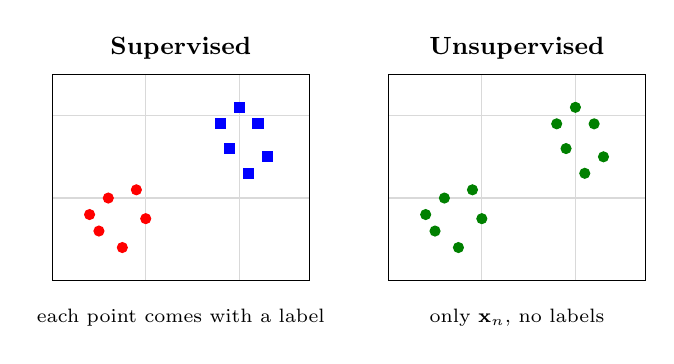
\begin{tikzpicture}
\begin{axis}[name=sup,
    width=0.4\linewidth, height=4.2cm,
    xmin=0, xmax=5.5, ymin=0, ymax=5, enlargelimits=false,
    grid=major, grid style={gray!30}, major tick length=0pt,
    xticklabels={}, yticklabels={},
    title={\small\textbf{Supervised}}, title style={yshift=-4pt},
    xlabel={\scriptsize each point comes with a label}, label style={font=\scriptsize}]
\addplot[only marks, mark=*, red, mark size=1.8pt] coordinates {(1,1.2) (1.5,0.8) (2,1.5) (1.2,2) (1.8,2.2) (0.8,1.6)};
\addplot[only marks, mark=square*, blue, mark size=1.8pt] coordinates {(3.8,3.2) (4.4,3.8) (4,4.2) (4.6,3) (3.6,3.8) (4.2,2.6)};
\end{axis}
\begin{axis}[at={(sup.east)}, anchor=west, xshift=1cm,
    width=0.4\linewidth, height=4.2cm,
    xmin=0, xmax=5.5, ymin=0, ymax=5, enlargelimits=false,
    grid=major, grid style={gray!30}, major tick length=0pt,
    xticklabels={}, yticklabels={},
    title={\small\textbf{Unsupervised}}, title style={yshift=-4pt},
    xlabel={\scriptsize only $\mathbf{x}_n$, no labels}, label style={font=\scriptsize}]
\addplot[only marks, mark=*, green!50!black, mark size=1.8pt] coordinates {(1,1.2) (1.5,0.8) (2,1.5) (1.2,2) (1.8,2.2) (0.8,1.6) (3.8,3.2) (4.4,3.8) (4,4.2) (4.6,3) (3.6,3.8) (4.2,2.6)};
\end{axis}
\end{tikzpicture}
\par}
